
\chapter{Architecture Assumptions}

We have built the module based on following disaggregation architecture. 
A server has a small amount of local memory. Rest of the memory is located on remote memory "blade". When CPU needs to access an address from an address space which is located on remote memory, it requests it though standard hardware protocol. High speed network interconnection is used to setup communication between devices. A local page is evicted based on the eviction policy. Then the requested remote page is transferred over the network to the local memory. 

\begin{figure}[tbp]
  \centering
    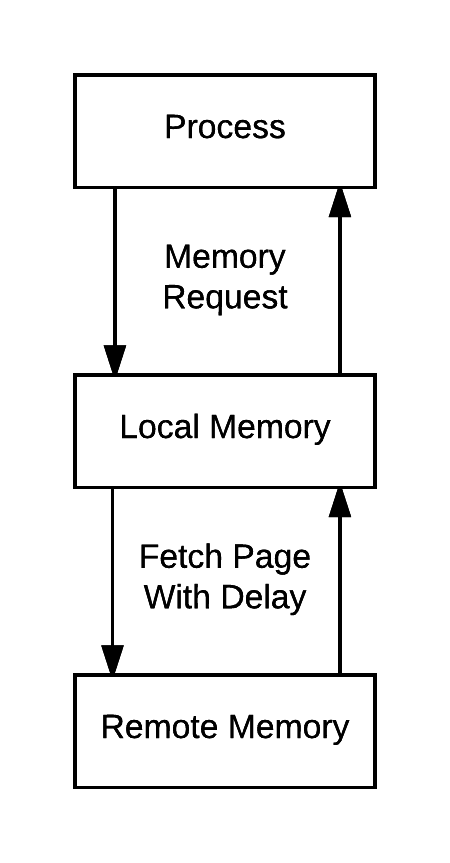
\includegraphics[width=0.25\textwidth]{assumption/architecture_assumption}
    \caption[Disaggregated Memory Flow]{Disaggregated memory flow.}
    \label{fig:arch} 
\end{figure}

%%% Local Variables: 
%%% mode: latex
%%% TeX-master: "../mainrep"
%%% End: 
